\documentclass[12pt]{scrartcl}\usepackage[]{graphicx}\usepackage[]{color}
%% maxwidth is the original width if it is less than linewidth
%% otherwise use linewidth (to make sure the graphics do not exceed the margin)
\makeatletter
\def\maxwidth{ %
  \ifdim\Gin@nat@width>\linewidth
    \linewidth
  \else
    \Gin@nat@width
  \fi
}
\makeatother

\definecolor{fgcolor}{rgb}{0.345, 0.345, 0.345}
\newcommand{\hlnum}[1]{\textcolor[rgb]{0.686,0.059,0.569}{#1}}%
\newcommand{\hlstr}[1]{\textcolor[rgb]{0.192,0.494,0.8}{#1}}%
\newcommand{\hlcom}[1]{\textcolor[rgb]{0.678,0.584,0.686}{\textit{#1}}}%
\newcommand{\hlopt}[1]{\textcolor[rgb]{0,0,0}{#1}}%
\newcommand{\hlstd}[1]{\textcolor[rgb]{0.345,0.345,0.345}{#1}}%
\newcommand{\hlkwa}[1]{\textcolor[rgb]{0.161,0.373,0.58}{\textbf{#1}}}%
\newcommand{\hlkwb}[1]{\textcolor[rgb]{0.69,0.353,0.396}{#1}}%
\newcommand{\hlkwc}[1]{\textcolor[rgb]{0.333,0.667,0.333}{#1}}%
\newcommand{\hlkwd}[1]{\textcolor[rgb]{0.737,0.353,0.396}{\textbf{#1}}}%

\usepackage{framed}
\makeatletter
\newenvironment{kframe}{%
 \def\at@end@of@kframe{}%
 \ifinner\ifhmode%
  \def\at@end@of@kframe{\end{minipage}}%
  \begin{minipage}{\columnwidth}%
 \fi\fi%
 \def\FrameCommand##1{\hskip\@totalleftmargin \hskip-\fboxsep
 \colorbox{shadecolor}{##1}\hskip-\fboxsep
     % There is no \\@totalrightmargin, so:
     \hskip-\linewidth \hskip-\@totalleftmargin \hskip\columnwidth}%
 \MakeFramed {\advance\hsize-\width
   \@totalleftmargin\z@ \linewidth\hsize
   \@setminipage}}%
 {\par\unskip\endMakeFramed%
 \at@end@of@kframe}
\makeatother

\definecolor{shadecolor}{rgb}{.97, .97, .97}
\definecolor{messagecolor}{rgb}{0, 0, 0}
\definecolor{warningcolor}{rgb}{1, 0, 1}
\definecolor{errorcolor}{rgb}{1, 0, 0}
\newenvironment{knitrout}{}{} % an empty environment to be redefined in TeX

\usepackage{alltt}
\usepackage[top=1in, bottom= 1in, left= 1in, right= 1in]{geometry}
\usepackage[USenglish]{babel} % set the language; greek allows \textgreek{\euro}
\usepackage{multirow} % For tables
\usepackage{graphicx, subfigure} % For graphics
\usepackage{setspace} % allows for vsape
\usepackage{natbib} % package to organize literature --> google it!
\usepackage{verbatim} % For including R-code
\usepackage{booktabs} % nicer tables
\usepackage{alltt} % verbatim + highlighting
\usepackage{amsmath} %boldsymbols
\usepackage{lscape} %Querformat
\usepackage{dcolumn} % align at decimal mark
\usepackage{floatrow} % description paragraphs below figures and tables
\usepackage{enumerate} % alter enumerate items (i,ii,iii etc)
\usepackage[colorlinks=true,citecolor=blue,urlcolor=blue]{hyperref}
\usepackage{amsfonts}
\setlength{\headheight}{15pt}
% http://en.wikibooks.org/wiki/LaTeX/Page_Layout for additional info

\title{Comparison of the Efficiency of Majority Election Results}
\subtitle{Part 4: Effects of Skewness, Ideal Point Scenarios, and Analytical Solutions}
\author{}
\IfFileExists{upquote.sty}{\usepackage{upquote}}{}

\begin{document}
\maketitle

\section{Simulating the Effect of Skewness}

\subsection{Keeping the Real Mean and Variance of Skewed Normal Distribution Constant}

The pdf of the skewed normal distribution is given by
\begin{equation}
f(x)=\dfrac{1}{\omega\pi}e^{-\tfrac{(x-\xi)^2}{2\omega^2}}
\int_{-\infty}^{\alpha\left(\tfrac{x-\xi}{\omega}\right)}
e^{-\tfrac{t^2}{2}}dt,
\end{equation}
where $\alpha \in \mathbb{R}$ is the \textit{shape} parameter (affecting skewness), $\xi \in \mathbb{R}$ is the \textit{location} parameter, and $\omega \in \mathbb{R^+}$ is the \textit{scale} parameter. Note that $\xi$ is not equal to the distribution's mean $\mu$, and $\omega$ is not it's variance $\sigma^2$. Rather, they are given by
\begin{align}
\mu &= \xi + \omega\dfrac{\alpha}{\sqrt{1+\alpha^2}}\sqrt{\dfrac{2}{\pi}} \\
\sigma^2 &= \omega^2 \left(1-\dfrac{2\left(\tfrac{\alpha}{\sqrt{1+\alpha^2}}\right)^2}{\pi}\right)
\end{align}
Accordingly, if we also want to keep the variance constant at $\sigma^{2*}$, we have to adjust the scale parameter such that:
\begin{equation}
\omega = \sqrt{\dfrac{\sigma^{2*}\pi}{\pi-2\left(\tfrac{\alpha}{\sqrt{1+\alpha^2}}\right)^2}}
\end{equation}
Furthermore, if we want to manipulate the skewness but keep the real mean of the distribution constant at $\mu^*$, we have to adjust the location parameter such that:
\begin{equation}
\xi = \mu^* - \omega\dfrac{\alpha}{\sqrt{1+\alpha^2}}\sqrt{\dfrac{2}{\pi}}
\end{equation}


\subsection{Overview of Simulation Parameters}
\begin{itemize}
\item Number of simulations for each scenario: 1000
\item Numbers of voters: 10, 20, 50, 100, 200, 500, 1000, 2000, 5000, 10000
\item Utility distributions for each voter (candidates $A$ and $B$): \\
$U_A \sim \mathcal{N}(\mu=0+\epsilon,\sigma^2=1)$ \\
$U_B \sim \mathcal{N}_{skew}\left(\xi=-\epsilon- \omega\dfrac{\alpha}{\sqrt{1+\alpha^2}}\sqrt{\dfrac{2}{\pi}},
\omega=\sqrt{\dfrac{\pi}{\pi-2\left(\tfrac{\alpha}{\sqrt{1+\alpha^2}}\right)^2}}\right)$
\item Differences in distribution means ($\epsilon$): -1, -0.75, -0.5, -0.25, -0.05, -0.025, -0.01, -0.005, 0, 0.005, 0.01, 0.025, 0.05, 0.1, 0.25, 0.5, 0.75, 1
\item Skewness of distribution ($\alpha$): 0, 1, 2, 5, 10
\item For now: no correlation between utilities
\end{itemize}

\clearpage
\subsection{Simulations}



\subsubsection{Skewness: alpha = 0}
\begin{knitrout}
\definecolor{shadecolor}{rgb}{0.969, 0.969, 0.969}\color{fgcolor}
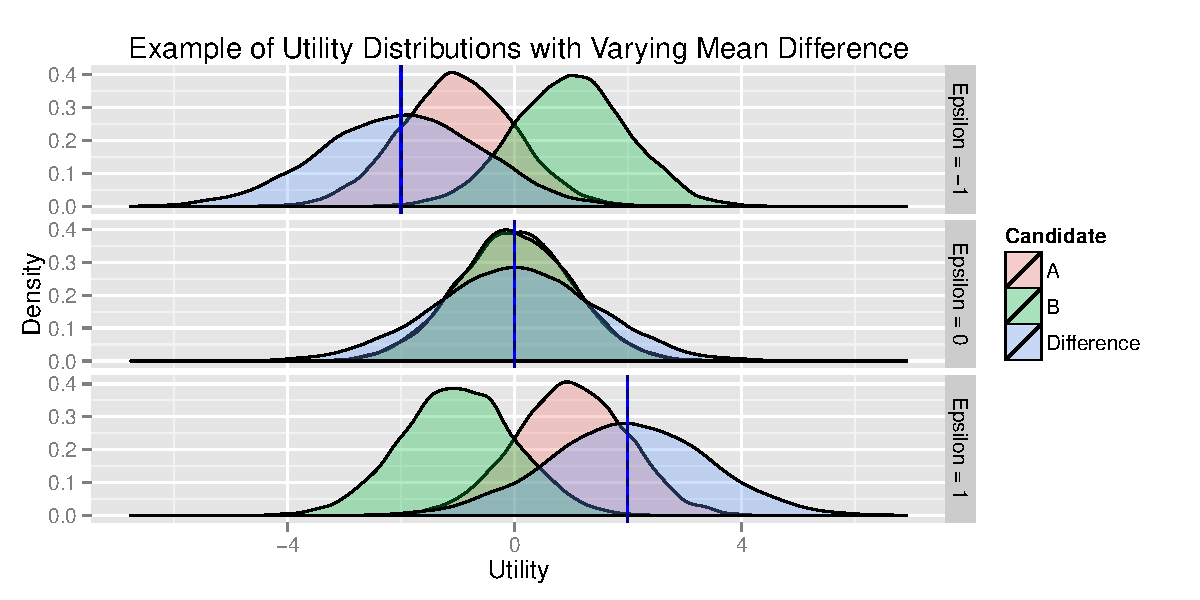
\includegraphics[width=\maxwidth]{figure/unnamed-chunk-2} 

\end{knitrout}


\begin{knitrout}
\definecolor{shadecolor}{rgb}{0.969, 0.969, 0.969}\color{fgcolor}
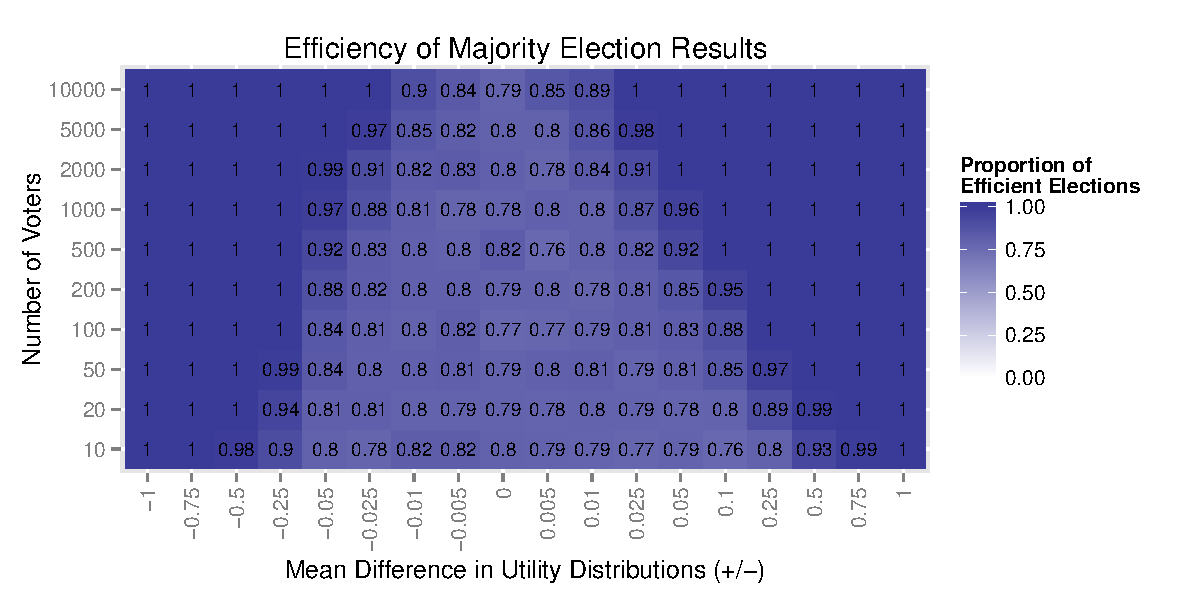
\includegraphics[width=\maxwidth]{figure/unnamed-chunk-3} 

\end{knitrout}


\clearpage
\subsubsection{Skewness: alpha = 1}
\begin{knitrout}
\definecolor{shadecolor}{rgb}{0.969, 0.969, 0.969}\color{fgcolor}
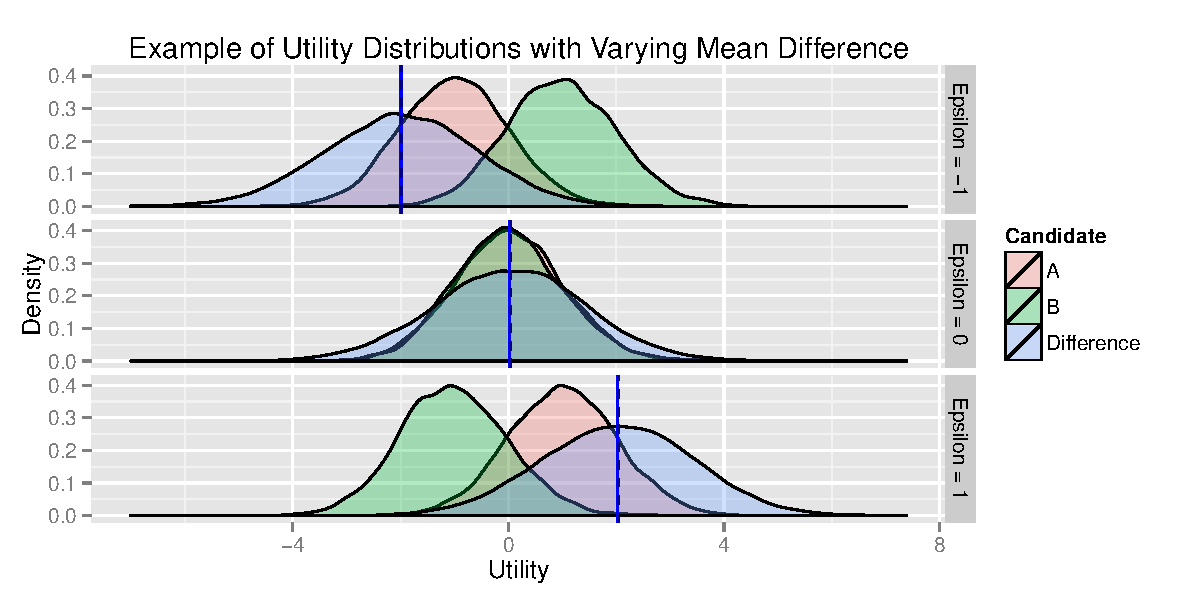
\includegraphics[width=\maxwidth]{figure/unnamed-chunk-4} 

\end{knitrout}


\begin{knitrout}
\definecolor{shadecolor}{rgb}{0.969, 0.969, 0.969}\color{fgcolor}
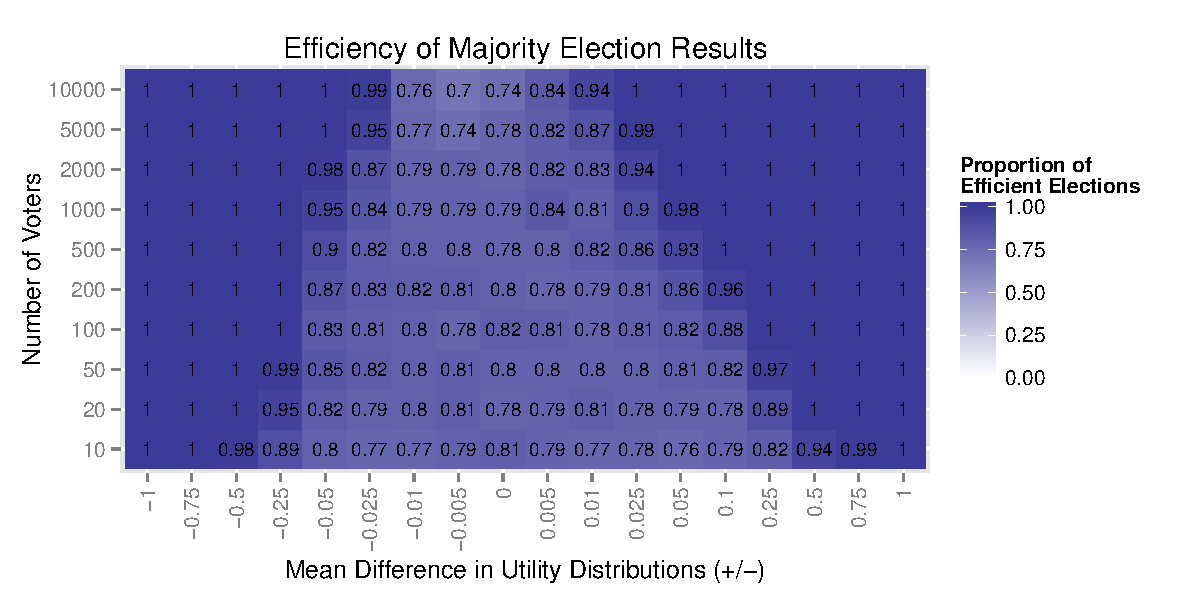
\includegraphics[width=\maxwidth]{figure/unnamed-chunk-5} 

\end{knitrout}


\clearpage
\subsubsection{Skewness: alpha = 2}
\begin{knitrout}
\definecolor{shadecolor}{rgb}{0.969, 0.969, 0.969}\color{fgcolor}
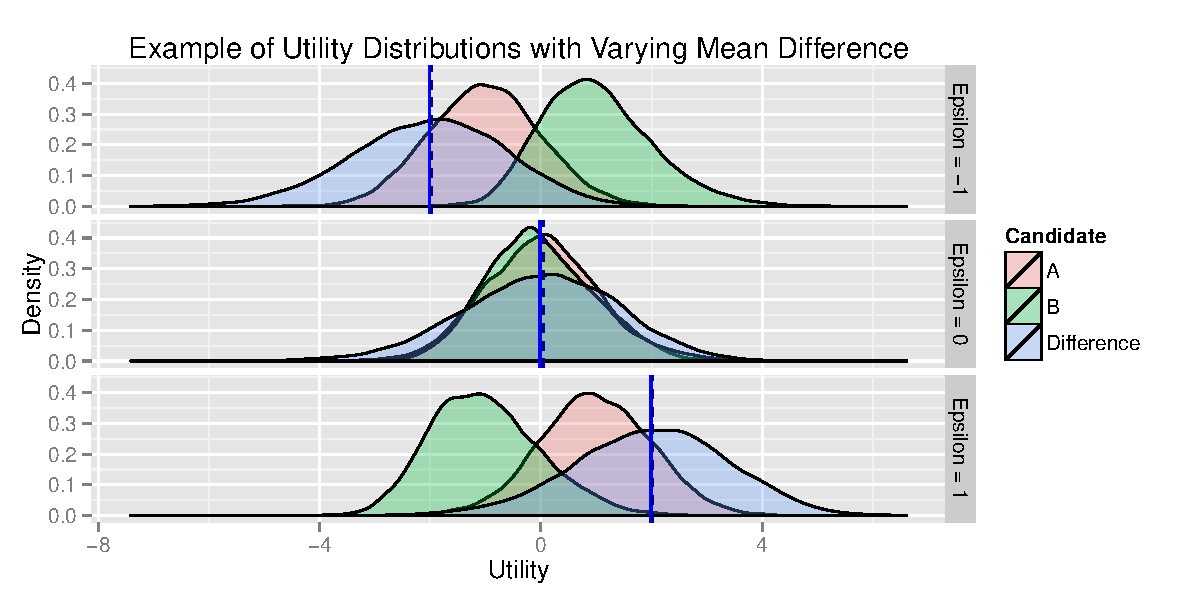
\includegraphics[width=\maxwidth]{figure/unnamed-chunk-6} 

\end{knitrout}


\begin{knitrout}
\definecolor{shadecolor}{rgb}{0.969, 0.969, 0.969}\color{fgcolor}
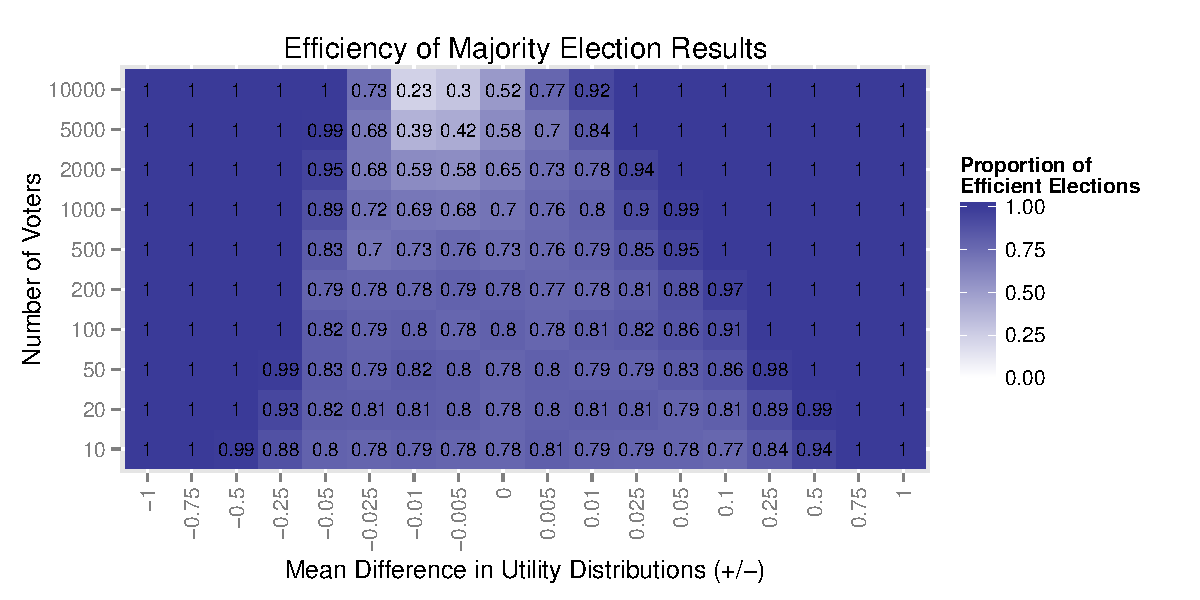
\includegraphics[width=\maxwidth]{figure/unnamed-chunk-7} 

\end{knitrout}


\clearpage
\subsubsection{Skewness: alpha = 5}
\begin{knitrout}
\definecolor{shadecolor}{rgb}{0.969, 0.969, 0.969}\color{fgcolor}
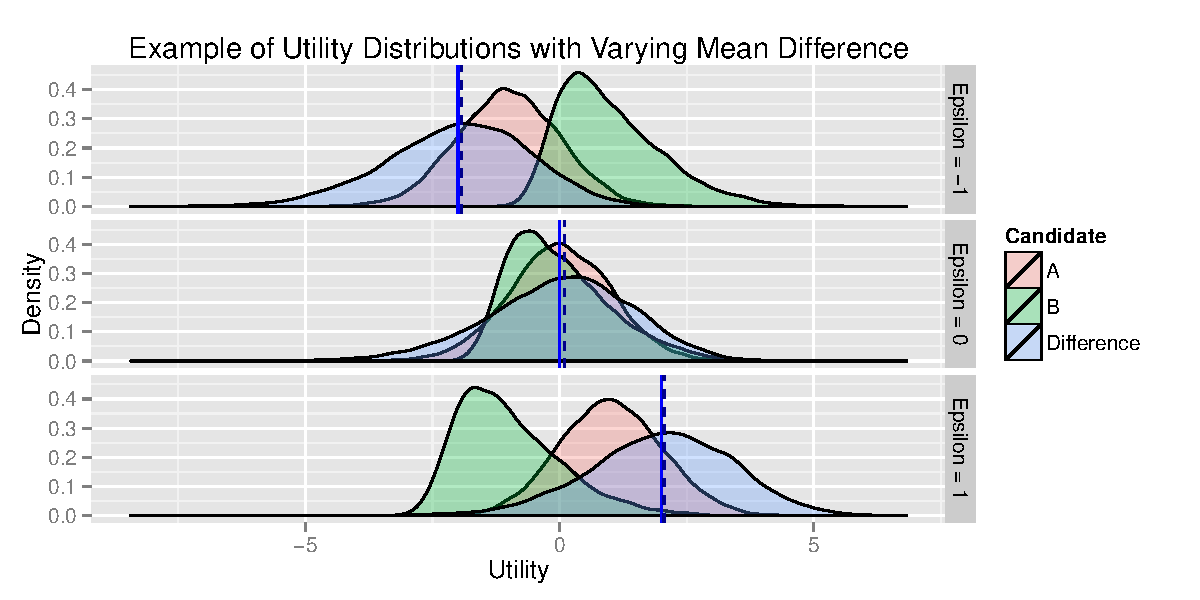
\includegraphics[width=\maxwidth]{figure/unnamed-chunk-8} 

\end{knitrout}


\begin{knitrout}
\definecolor{shadecolor}{rgb}{0.969, 0.969, 0.969}\color{fgcolor}
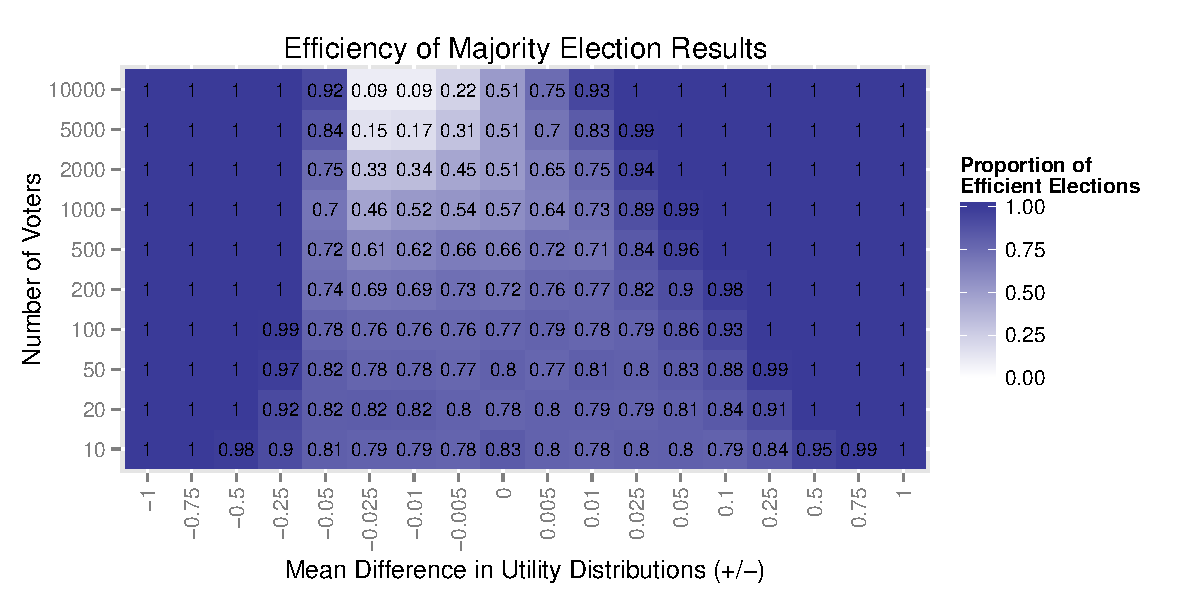
\includegraphics[width=\maxwidth]{figure/unnamed-chunk-9} 

\end{knitrout}


\clearpage
\subsubsection{Skewness: alpha = 10}
\begin{knitrout}
\definecolor{shadecolor}{rgb}{0.969, 0.969, 0.969}\color{fgcolor}
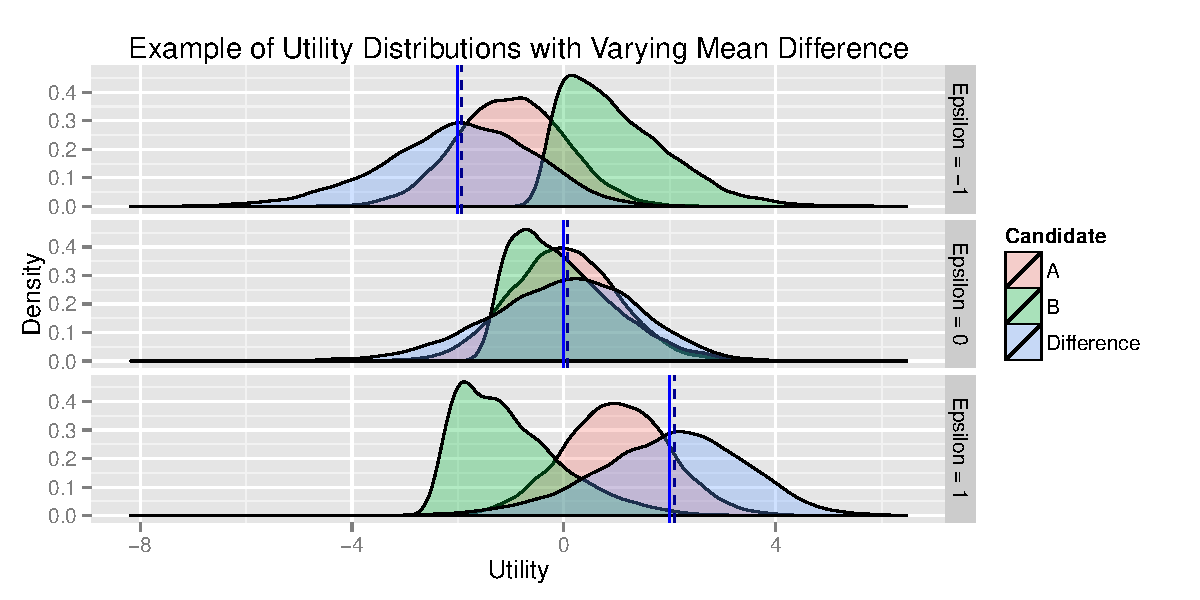
\includegraphics[width=\maxwidth]{figure/unnamed-chunk-10} 

\end{knitrout}


\begin{knitrout}
\definecolor{shadecolor}{rgb}{0.969, 0.969, 0.969}\color{fgcolor}
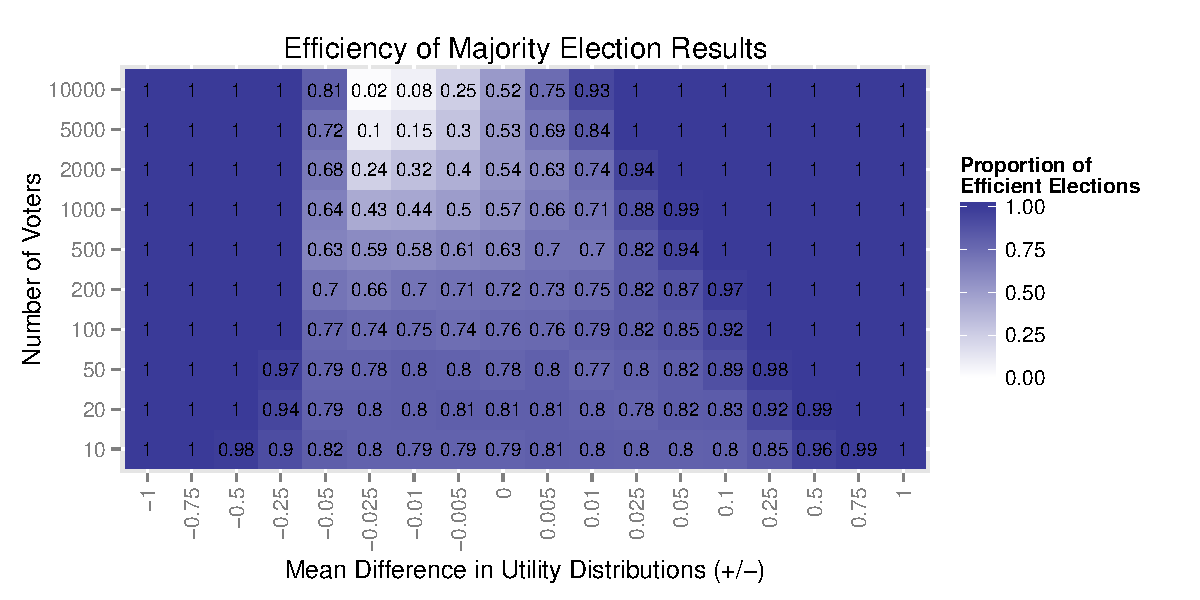
\includegraphics[width=\maxwidth]{figure/unnamed-chunk-11} 

\end{knitrout}


\clearpage
\section{Investigating Ideal Point Scenarios that Lead to Skewed Utility Differentials}
\begin{align*}
X_{cand1},X_{cand2} &\sim \mathcal{N}(\mu=0,\sigma^2=1) \\
X_i &\sim \mathcal{N}_{skew}\left(\xi=0- \omega\dfrac{\alpha}{\sqrt{1+\alpha^2}}\sqrt{\dfrac{2}{\pi}},
\omega=\sqrt{\dfrac{\pi}{\pi-2\left(\tfrac{\alpha}{\sqrt{1+\alpha^2}}\right)^2}}\right) \\
U_{i1,i2} &= -(X_{cand1,cand2}-X_i)^2
\end{align*}

\begin{knitrout}
\definecolor{shadecolor}{rgb}{0.969, 0.969, 0.969}\color{fgcolor}
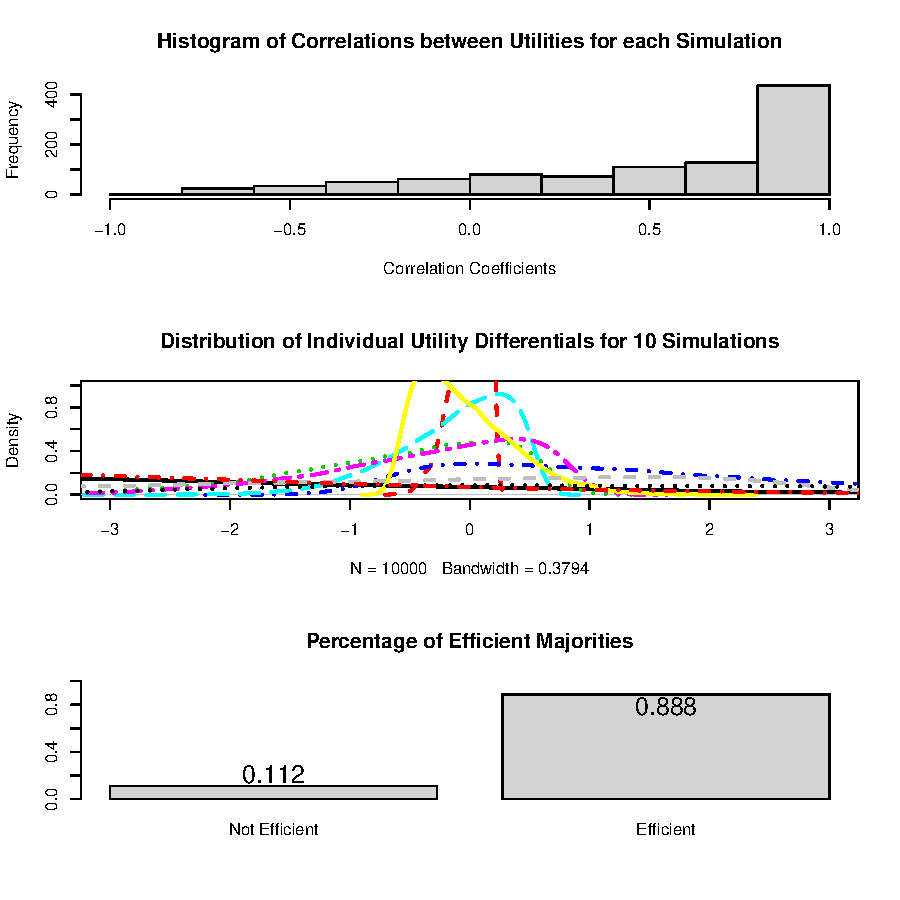
\includegraphics[width=\maxwidth]{figure/unnamed-chunk-12} 

\end{knitrout}


\section{Analytical Solution for Efficiency Probability (for non-skewed utilities)}

Coming next: assume that true mean difference is zero, and median falls on one side of the zero point or the other. What is the probability that the individuals on the opposite side outweigh the median side (in order to pull the mean on their side). This probability decreases with increasing sample size (relative size of groups on either side etc...)

\end{document}
